\section{Descripción de la Solución Propuesta}
Dada la problemática expuesta en la sección \ref{problem_statement}, en la que
se describe de manera breve el enfoque que se le piensa brindar, en esta sección
se trata de describir la primera aproximación a su solución de forma detallada.

Sin duda, la realización de una herramienta de software libre reutilizable para
la implementación de trámites y su correspondiente seguimiento a nivel de
backend tiene muchas ventajas, pero su realización no es del todo trivial y
demanda que se conceptualice en un modelo medianamente robusto, con metodologías
claras y descripciones escuetas.

Cuando uno piensa en trámites, usualmente piensa en burocracia, en largas filas,
una obligación muchas veces irrenunciable y una lista interminable de pasos a
seguir. Según la Real Academia de la Lengua Española, se define como \say{Cada
	uno de los pasos y diligencias que hay que recorrer en un asunto hasta su
	conclusión} \parencite{asaleDiccionarioLenguaEspanola}.

Si bien las definiciones de trámite son escasas y algunas pueden tratar su
semántica desde una perspectiva más funcional, es indudable que un trámite es un
procedimiento que consta de uno o más pasos a seguir. De este modo, se puede
vislumbrar una manera casi obvia de modelarlo usando conceptos de teoría
computacional, de matemáticas discretas o circuitos secuenciales. Esto es,
usando máquinas de estado finitas.

Este enfoque no es precisamente nuevo y ya se puede ver en una aproximación al
modelado en software de distintos trámites de la división de gestiones,
admisiones y registros de la UMSA, donde se emplearon máquinas de Turing que a
efectos prácticos se aproximan más a máquinas de estado finitas
\parencite{nachoSISTEMACONTROLTRAMITES2007}, como se puede ver en la figura
\ref{fig:nachocarreraparalela}.

\begin{figure}
	\centering
	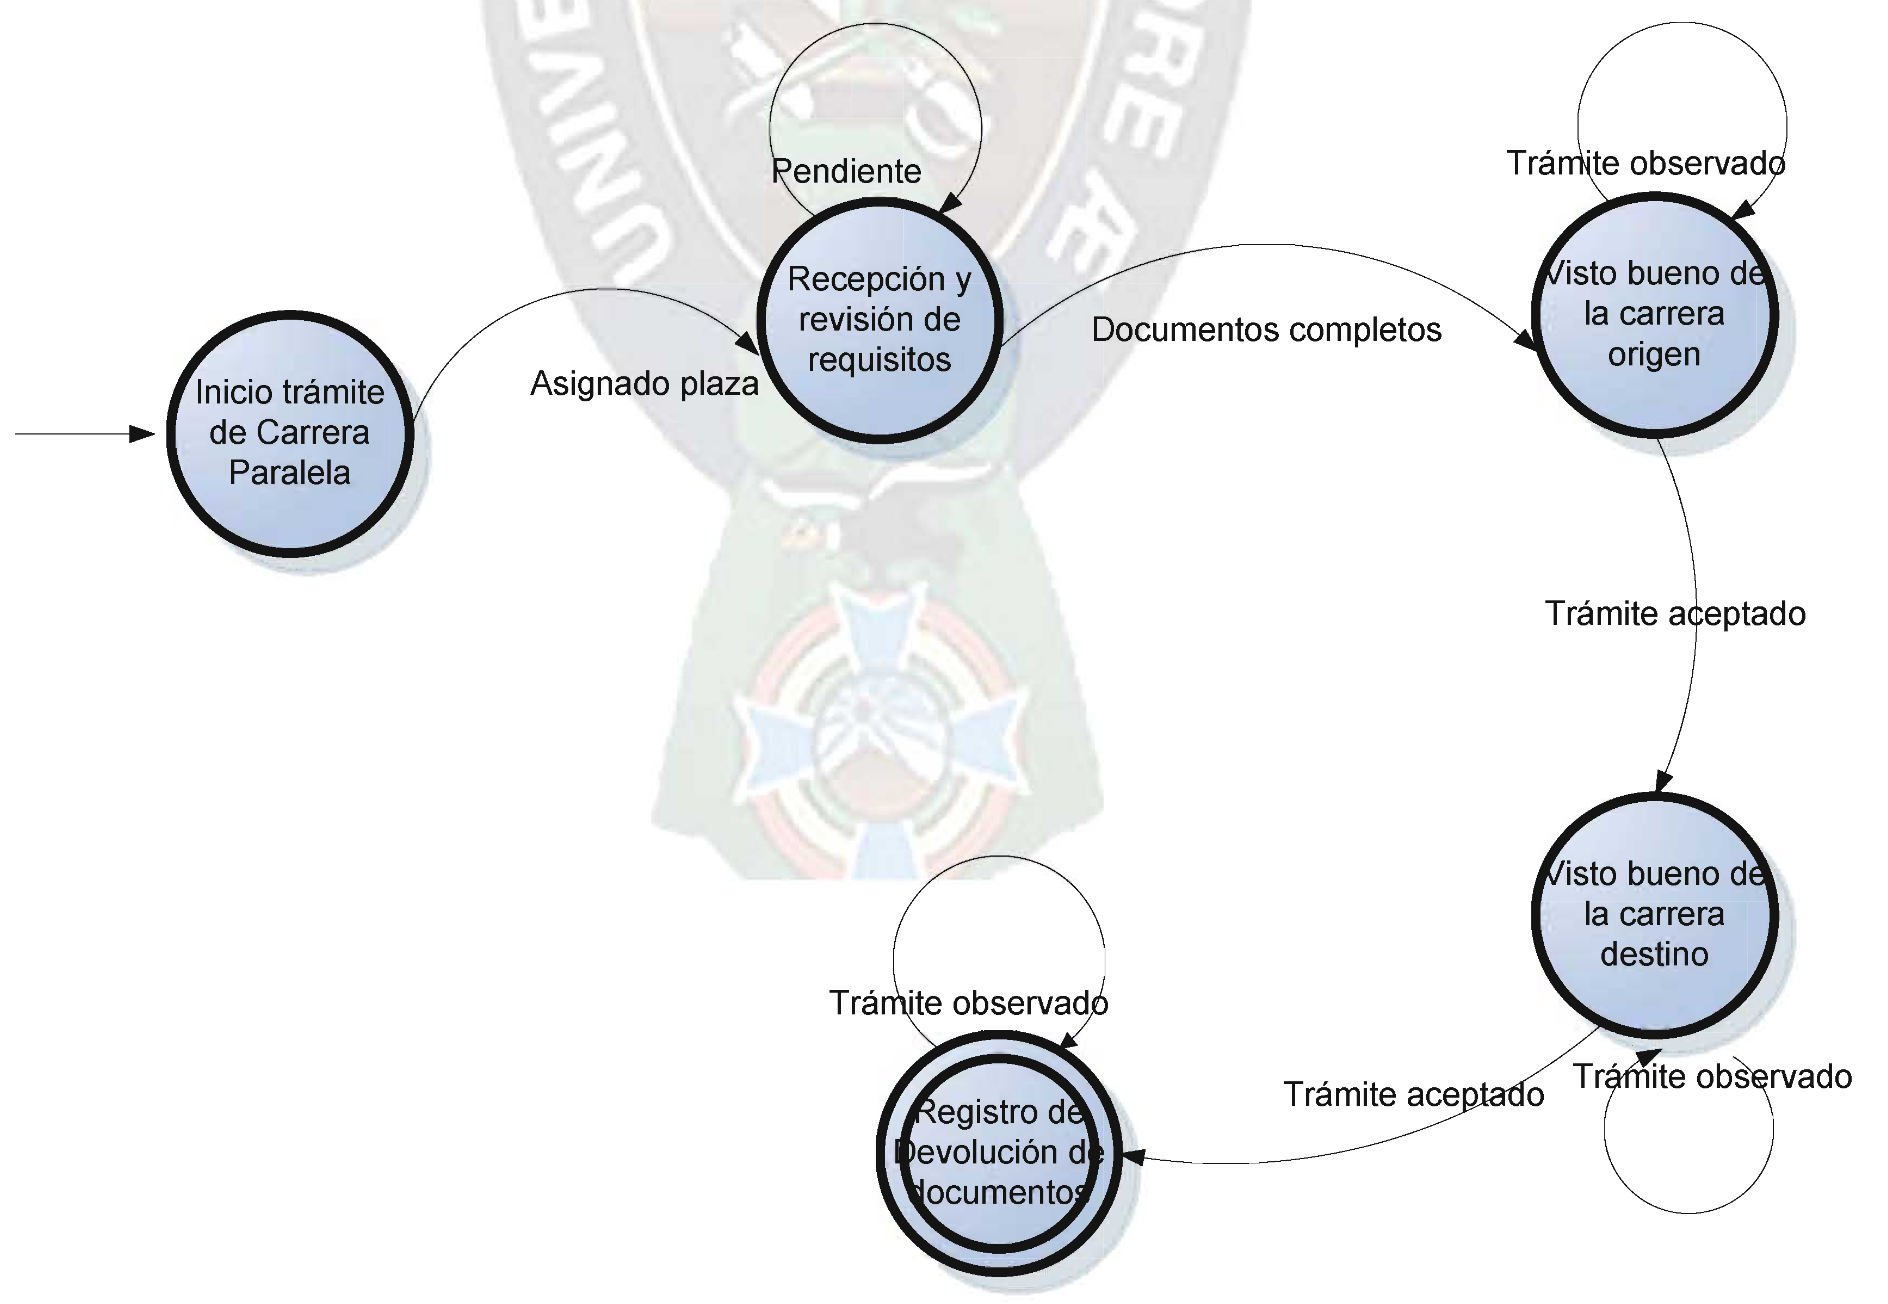
\includegraphics[width=0.7\textwidth]{assets/carreraparalelanacho}
	\caption{Diagrama de una máquina de Turing para carreras paralelas
		desarrollada en \cite{nachoSISTEMACONTROLTRAMITES2007}}
	\label{fig:nachocarreraparalela}
\end{figure}

Desde luego, las máquinas de estados finitas parecen ser una manera sencilla de
modelar los procesos de trámite a nivel de software, principalmente por su
paralelismo con los pasos y sus respectivas transiciones, asemejándose a un
procedimiento administrativo, como se puede evidenciar en la definición
matemática de este autómata:

\begin{definition}[Máquina de Estados Finita]
	Una máquina de estados es un conjunto de 5 elementos $M=(S,I,O,v,w)$, donde
	$S$ representa a la colección de estados de $M$; $I$ representa al alfabeto
	de entradas para M; O es el alfabeto de salidas de M; $v:SxI->S$ es la
	función del siguiente estado; y $w:SxI->O$ es la función de salida
	\parencite{grimaldiDiscreteCombinatorialMathematics1998}.
\end{definition}

Este paralelismo es más notorio en un diagrama de estados como el que se muestra
en la figura \ref{fig:states}, donde tenemos los estados de $S = (s_{0}, s_{1},
	s_{2}, s_{3}, s_{4}, s_{5}, s_{error})$ y algunas transiciones entre los mismos,
cada una con sus correspondientes entradas ($\iota_{mn}$) y salidas ($o_{mn}$).
Las transiciones restantes se omiten porque apuntan a un mismo estado de error
del trámite ($s_{error}$).

\begin{figure}[ht]
	\centering
	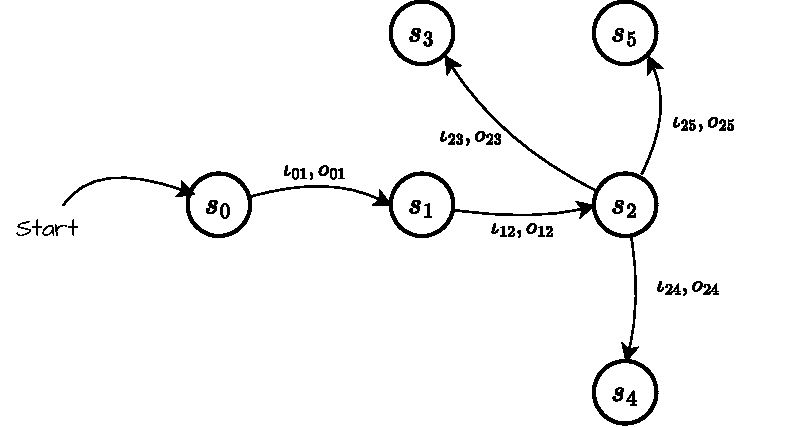
\includegraphics[width=0.8\textwidth]{assets/statediagramexample}
	\caption{Diagrama de estados finitos con salidas}
	\label{fig:states}
\end{figure}

En la figura \ref{fig:states_procedure} podemos ver el mismo diagrama, pero
simplificado y usando un lenguaje cercano a la naturaleza de los procedimientos
administrativos de forma adrede para hacer más obvia la relación descrita.
Nótese que se usan para los estados nombres cortos y no totalmente detallados
para fines prácticos de ilustración. En un sistema real se esperan definiciones
claras que reflejen la totalidad del trámite implementado.

\begin{figure}[ht]
	\centering
	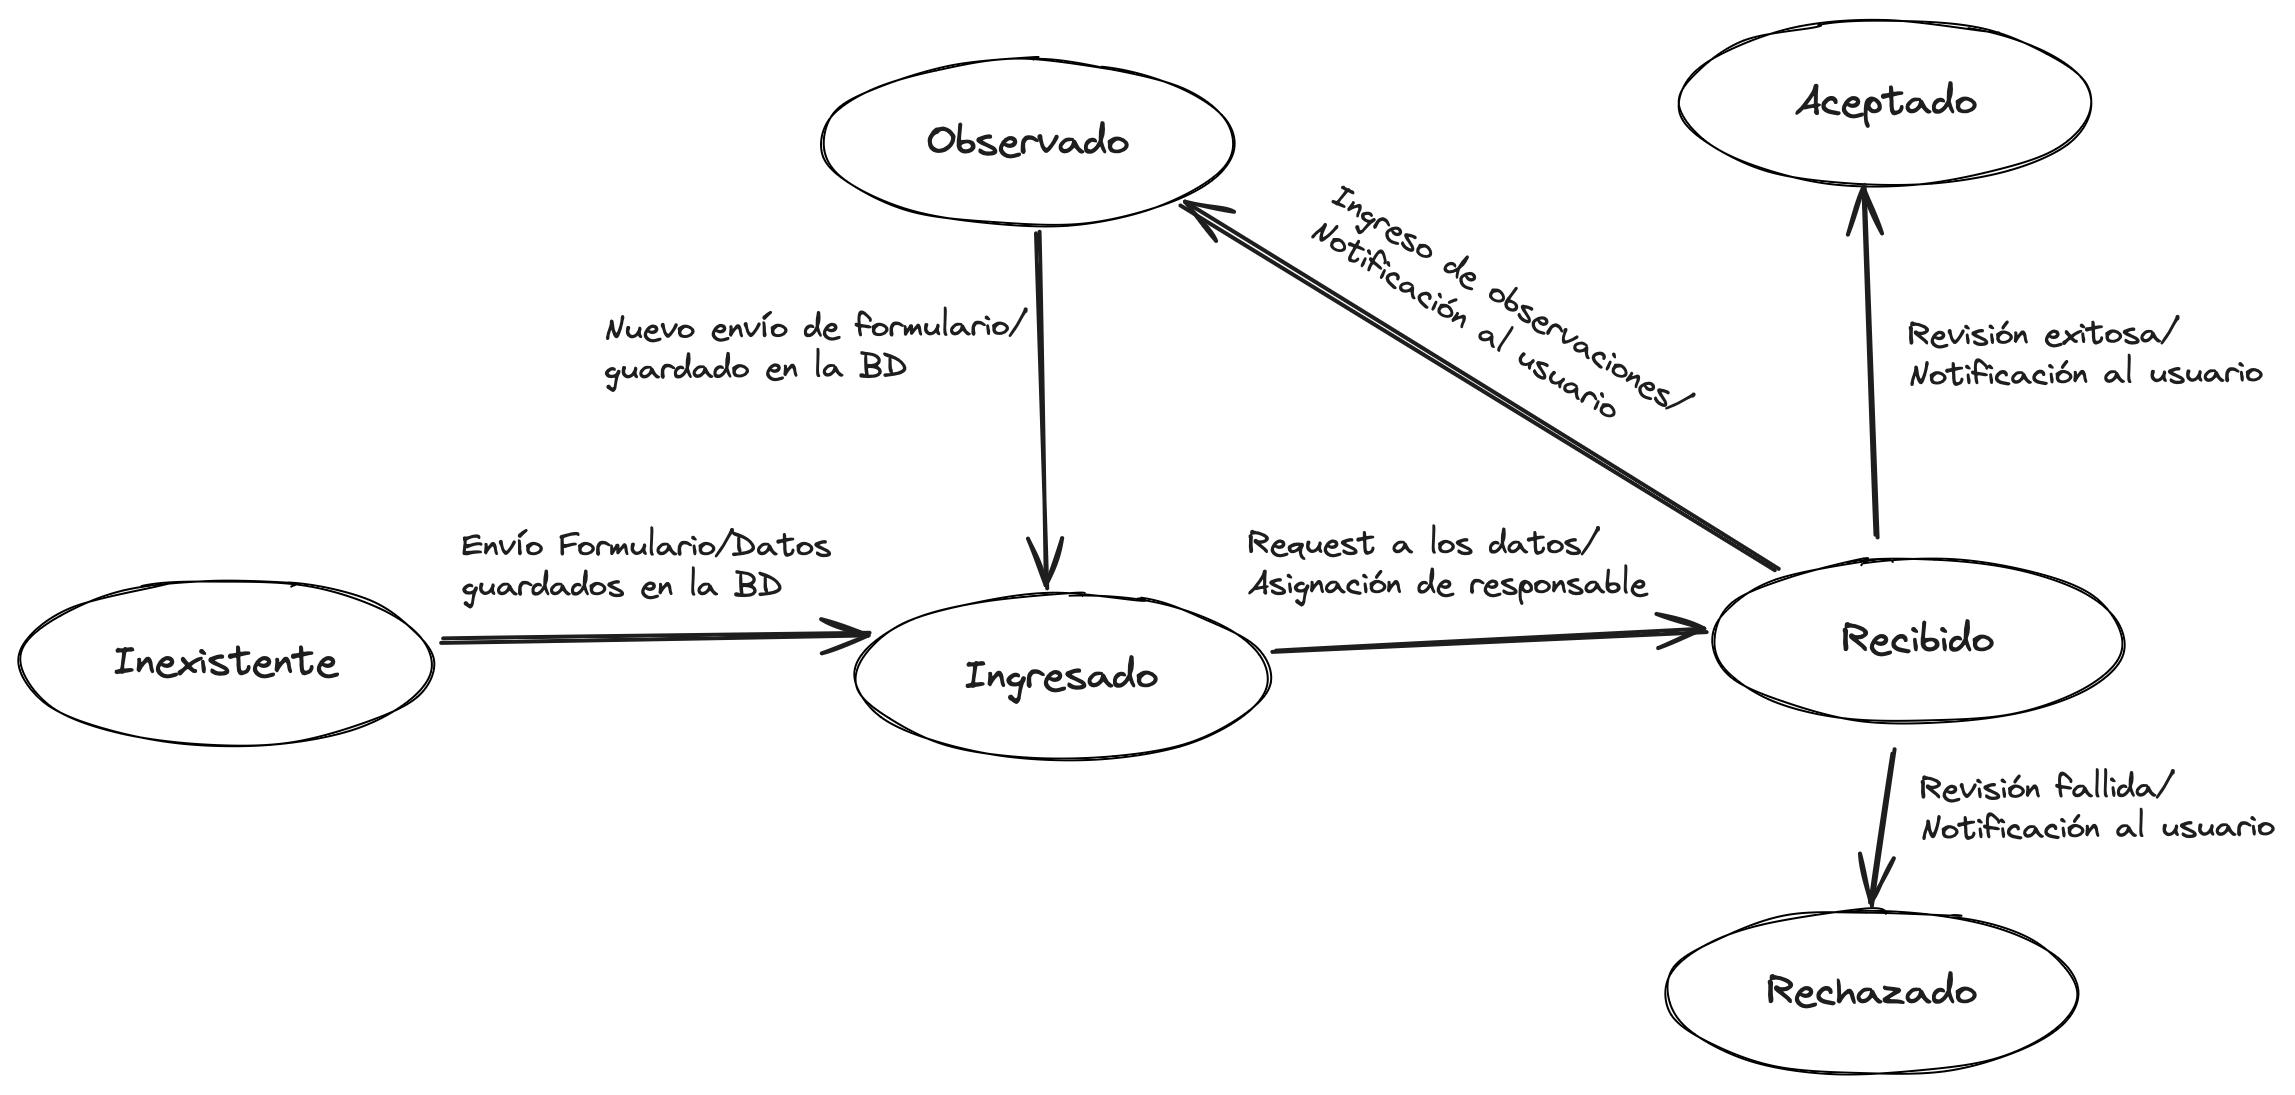
\includegraphics[width=0.8\textwidth]{assets/stateprocedureexample}
	\caption{Diagrama de estados simplificado para un trámite}
	\label{fig:states_procedure}
\end{figure}

Se plantea utilizar este enfoque del uso de autómatas, como también son llamadas
las máquinas de estado en contextos de teoría computacional, pero con ciertos
lineamientos conceptuales que guíen al usuario de esta solución, que
inicialmente serían:

\begin{itemize}
	\item Descripción detallada de los estados, compuesta mínimamente por un
	      nombre único, una descripción, el sujeto cuya perspectiva se usa para la
	      descripción y su visibilidad.

	\item Preferencia del autómata de Moore sobre el autómata de Mealy. Los
	      autómatas de Mealy son una simplificación en número de estados a partir
	      de los autómatas de Moore, con estados que en las aplicaciones
	      originales del concepto podían ser considerados innecesarios
	      \parencite{mealyMethodSynthesizingSequential1955}.  Si bien en muchas
	      aplicaciones es lo deseado, en temas de auditoría se prefiere tener la
	      mayor cantidad de información relevante, por lo que sin restringir el
	      uso de máquinas de Mealy, se priorizará el uso de máquinas de Moore.

	\item Respecto al anterior punto, incluso si el usuario usa Mealy en lugar
	      de Moore, se recomienda la definición de tantos estados como sean
	      posibles.

	      % TODO: Aquí irían las definiciones de inputs, outputs, etc como lo tengo
	      % descrito en el Obsidian
\end{itemize}

Como parte de la solución propuesta, se debe entender que los lineamientos
conceptuales son muy importantes, ya que este proyecto no será solamente de
código abierto, sino además de concepto abierto, es decir, estas ideas se pueden
aplicar en otros entornos distintos al que se elegirá para esta solución
\cite[439]{sommervilleSoftwareEngineering2016}, el cual se detalla más adelante.

Cualquier implementación de software implica una toma detallada de
requerimientos sobre la cual trabajar. Quizá una desventaja del software libre
en la práctica es que las metodologías no son aplicadas correctamente, los
programadores definen los requerimientos y no hay objetivos medibles
\cite[Tabla~1]{aberdourAchievingQualityOpenSource2007}; esto debido a que no
existen las figuras de cliente, inversión y beneficio económico, que
precisamente son la fuente de los requerimientos más importantes para el
proyecto.

Por esto mismo, para la solución planteada se aprovechará el ya existente
proyecto SIAI (Sistema Integral Ambiental Industrial) del Viceministerio de
Desarrollo Productivo, desarrollado por la empresa 2IES y en el cual, el autor
de este documento, tuvo participación. Este sistema contempla requerimientos
comunes en la realización de trámites gubernamentales y será una guía para la
implementación actual.

Evidentemente, al ser un proyecto de código libre y al pretender dejar su
desarrollo abierto desde el día 1 en Github, sería un despropósito no aprovechar
y/o buscar más proyectos similares que puedan enriquecer el desarrollo actual.

El sistema SIAI, que será empleado como referencia, tendrá además otro papel
importante en este proyecto, siendo el producto del mismo utilizado en una
implementación de un fork del mencionado software para demostrar la usabilidad
del paquete.

Esto nos obliga a tomar una decisión a priori sobre el desarrollo del producto
que se propone como solución y es que, como cualquier otro paquete de software,
su implementación suele estar restringida a alguna tecnología existente
\cite[444]{sommervilleSoftwareEngineering2016}.  Dada la popularidad del
framework Laravel de PHP y a que el sistema SIAI está desarrollado usando estas
tecnologías se procederá a la creación de un paquete, precisamente, de Laravel.

La solución, al ser un paquete de software, contará no solamente con las ideas y
marcos de trabajo descritos anteriormente, sino que además se piensa brinde
herramientas que ayuden al proceso de trámites, como por ejemplo:

\begin{itemize}
	\item Generación de códigos de trámite.

	\item Generación de códigos de verificación de correos (Que si bien hay
	      alternativas para lo mismo, se facilitará el uso desde el paquete).

	\item Funcionalidad de notificaciones.

	\item Límites de tiempo asignables a los estados de trámite.

	\item Funcionalidad de persistencia de historial de estados incorporada.

	\item Funciones de recuperación de historia de trámite para seguimiento.

	\item Niveles de visibilidad de trámites para seguimiento.

	\item Mecanismos para dificultar el entorpecimiento de un trámite y
	      facilitar la identificación de responsables.

	\item Interfaz sencilla para cambio de estados de una máquina (trámite).
\end{itemize}

Para concluir esta aproximación a la solución a realizar, quedan dos puntos
importantes a tocar, uno de ellos opcional a la fecha de redacción de este
documento, y es acerca de la naturaleza FLOSS o FOSS de este proyecto.

Para que un proyecto de software sea considerado de software libre debe cumplir
con 4 libertades esenciales \cite{QueEsSoftware}:

\begin{itemize}
	\item La libertad de ejecutar el programa como se desee, con cualquier
	      propósito (libertad 0).

	\item La libertad de estudiar cómo funciona el programa, y cambiarlo para
	      que haga lo que se desee (libertad 1). El acceso al código fuente es una
	      condición necesaria para ello.

	\item La libertad de redistribuir copias para ayudar a otros (libertad 2).

	\item La libertad de distribuir copias de sus versiones modificadas a
	      terceros (libertad 3). Esto le permite ofrecer a toda la comunidad la
	      oportunidad de beneficiarse de las modificaciones. El acceso al código
	      fuente es una condición necesaria para ello.
\end{itemize}

Esto debe ser claramente definido en un documento de licencia de Software que se
encuentre junto al código fuente. Existen varias licencias que cumplen con los
lineamientos antes señalados y son aprobados por la FSF (Free Software
Foundation) \cite{VariousLicensesComments}.

Si bien la licencia predilecta del Software Libre es la GNU-GPL, de la cual
existe incluso una versión boliviana llamada LPG-Bolivia
\cite{cayoLPGBoliviaADSIB}, puede ser demasiado restrictiva para quien quiera
usar los resultados de este proyecto. Por esto mismo se piensa licenciar no sólo
el software sino también los documentos de proyecto asociados bajo alguna
licencia similar a la del MIT \cite{MITLicense2006}, que brinda la posibilidad
de generar software no libre a partir de software libre y es ampliamente usado
por varios proyectos Open Source.

Un proyecto de software libre suele ser distribuido en la red y suele tener
alguna denominación distintiva. Dada la naturaleza de los trámites, que consiste
en una secuencia de pasos se piensa bautizar al paquete resultante de este
proyecto como \say{Tunkunia}.